\section{Bakti QIlan Mufid (1174083)}
\subsection{Tugas Membuat Shapefile dengan PySHP}
\begin{enumerate}
	\item No 1
	\lstinputlisting{src/tugas2/1174083/scriptNo1.py}
	\begin{figure}[H]
		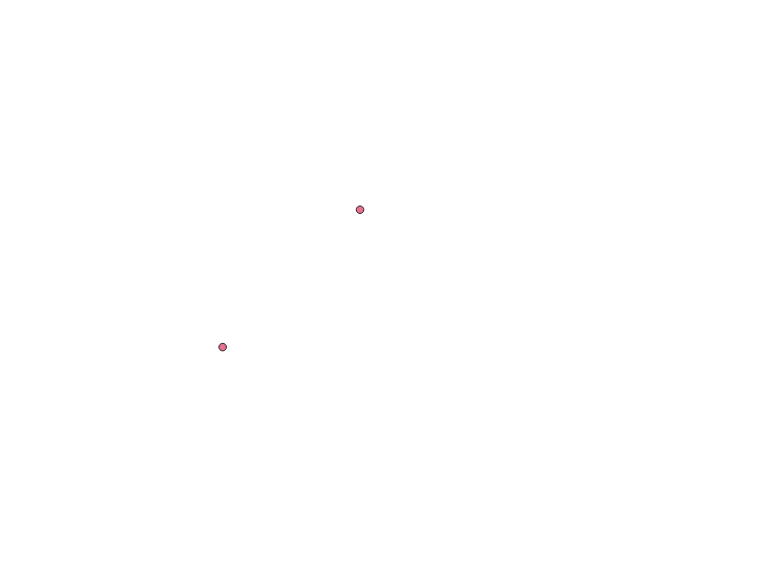
\includegraphics[width=6cm]{figures/Tugas2/1174083/1.png}
		\centering
		\caption{Hasil No 1}
	\end{figure}
	
	\item No 2
	\lstinputlisting{src/tugas2/1174083/scriptNo2.py}
	\begin{figure}[H]
		
\includegraphics[width=6cm]{figures/Tugas2/1174083/2.png}
		\centering
		\caption{Hasil No 2}
	\end{figure}

	\item No 3
	\lstinputlisting{src/tugas2/1174083/scriptNo3.py}
	\begin{figure}[H]
		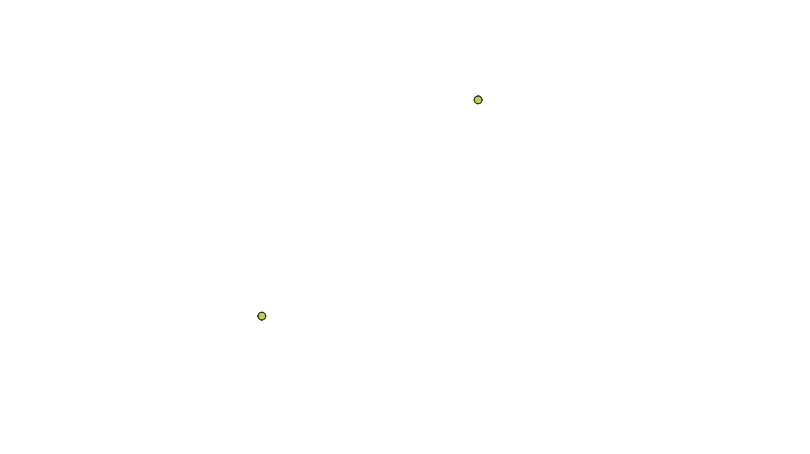
\includegraphics[width=6cm]{figures/Tugas2/1174083/3.png}
		\centering
		\caption{Hasil No 3}
	\end{figure}

	\item No 4
	\lstinputlisting{src/tugas2/1174083/scriptNo4.py}
	\begin{figure}[H]
		
\includegraphics[width=6cm]{figures/Tugas2/1174083/4.png}
		\centering
		\caption{Hasil No 4}
	\end{figure}

	\item No 5
	\lstinputlisting{src/tugas2/1174083/scriptNo5.py}
	\begin{figure}[H]
		
\includegraphics[width=6cm]{figures/Tugas2/1174083/5.png}
		\centering
		\caption{Hasil No 5}
	\end{figure}
	
	\item No 6
	\lstinputlisting{src/tugas2/1174083/scriptNo6.py}
	\begin{figure}[H]
		
\includegraphics[width=6cm]{figures/Tugas2/1174083/6.png}
		\centering
		\caption{Hasil No 6}
	\end{figure}

	\item No 7
	\lstinputlisting{src/tugas2/1174083/scriptNo7.py}
	\begin{figure}[H]
		
\includegraphics[width=6cm]{figures/Tugas2/1174083/7.png}
		\centering
		\caption{Hasil No 7}
	\end{figure}
	
	\item No 8
	\lstinputlisting{src/tugas2/1174083/scriptNo8.py}
	\begin{figure}[H]
		
\includegraphics[width=6cm]{figures/Tugas2/1174083/8.png}
		\centering
		\caption{Hasil No 8}
	\end{figure}

	\item No 9
	\lstinputlisting{src/tugas2/1174083/scriptNo9.py}
	\begin{figure}[H]
		
\includegraphics[width=6cm]{figures/Tugas2/1174083/9.png}
		\centering
		\caption{Hasil No 9}
	\end{figure}

	\item No 10
	\lstinputlisting{src/tugas2/1174083/scriptNo10.py}
	\begin{figure}[H]
		
\includegraphics[width=6cm]{figures/Tugas2/1174083/10.png}
		\centering
		\caption{Hasil No 10, NPM saya adalah 1174083, maka hasil modulus 8 dari NPM 1174083 adalah 3, jadi membuat bidang persegi panjang dan angka kedua terakhir di NPM saya dalah 8 maka saya akan membuat 8 buah persegi panjang}
	\end{figure}	
	
\end{enumerate}
\subsection{Link}
	https://youtu.be/XH4kwqY-fUE